\documentclass[systemskiss/skiss.tex]{subfiles}

\begin{document}

\section{Översikt av projektet}
Projektet kommer vara uppdelat i olika delar. Nedan följer en beskrivning av hur delarna ska se ut.
\subsection{Blockschema}
\begin{figure}[h]
    \centering
    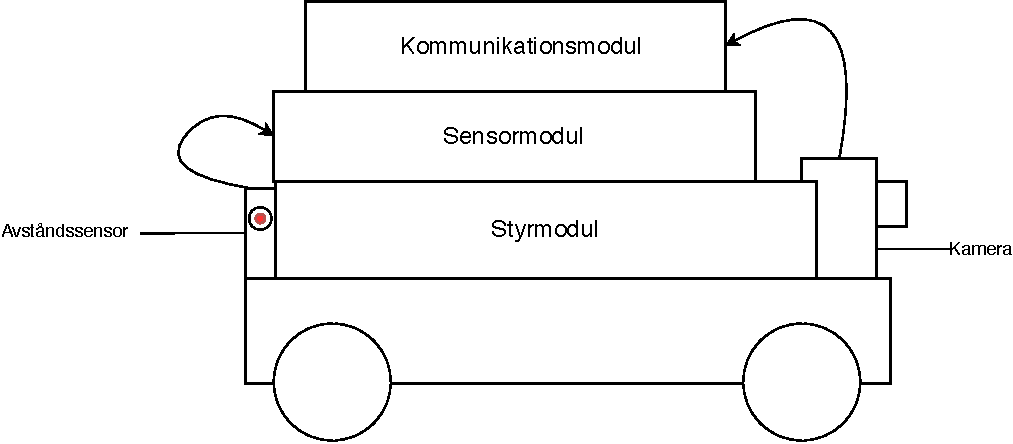
\includegraphics[width=0.6\linewidth]{systemskiss/figures/taxibilen.pdf}
    \caption{Enkel bild av systemets struktur}
    \label{fig:taxiskiss}
\end{figure}

Figur \ref{fig:taxiskiss} är en bild på hur hela systemet ska se ut när det är färdigmonterat. De tre modulerna är kopplade via en databuss. Figuren visar även vart kameran och sensorerna ska kopplas in. 
\subsection{Delsystem och gränssnitt}
Systemet kan främst delas in i moduler, men alla delar kommer inte behöva det. De blir istället delsystem. Kameran är ett delsystem eftersom den inte ingår i någon modul. På samma sätt är den bärbara datorn ett delsystem som trådlöst ska vara kopplad till bilen. 

\subsection{Modularitet och uppgraderbarhet}
Sytemet ska vara moduluppbyggt vilket innebär att man ska kunna byta ut vilken modul som helst mot en annan utan att systemet ska sluta fungera. Efter att systemet är färdigställt ska det också vara lätt att lägga till nya moduler efter behov. Därför ska modulerna kopplas samman med ett bestämt gränssnitt. 

\end{document}

